\section{Experimental Demonstration}\label{sec: experiments}
Consider a learner agent that is tasked with finding an optimal path
for supply transportation between point $S$ and $T$ on a grid. The
learner's reward is initially fixed to be $-1$ for every step it takes
plus some values $R_{ST}$ and $R_{TS}$ for reaching point T from S and
vice versa. In a uniform grid this would be a simple problem, however,
the grid simulates a terrain and cells have an associated elevation.  
As a result, any movement from one cell to another neighbouring cell
succeeds with a probability proportional to the relative elevation of 
the cells. Consider the situation depicted in Figure~\ref{exp_motion}. 

\begin{figure}[ht]
\centerline{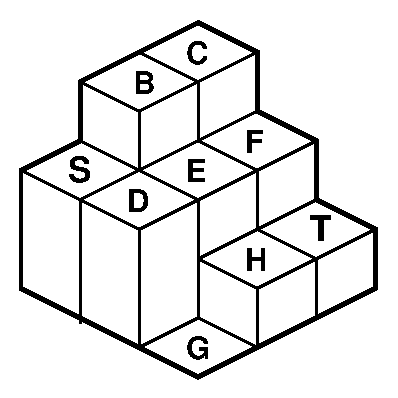
\psfig{file=img/exp_motion.eps,width=5cm}}
\caption{\label{exp_motion}Example of a 3D terrain grid}
\end{figure}

If the cells are of equal elevation, the movement almost always
succeeds, e.g. moving from cell $B$ to cell $C$ in
Figure~\ref{exp_motion}. If the source cell of the motion is lower
than the target cell, then the motion succeeds with low
probability. Furthermore, in this case, a non-zero probability exists
that the direction of motion will be altered. E.g. moving from $H$ to
$E$ is unlikely to succeed, and the agent may end up in $D$, $F$ or
even $G$. If the motion is directed to lower the elevation, it is most
likely will succeed, but also has certain probability to move further
than intended. E.g. moving from $B$ to $E$ is likely to succeed, but
the agent may end up in $H$ or $G$.

Finding an optimal path of motion from $S$ to $T$ and back is,
therefore, becomes non-trivial. Still, if the probabilities of
different transitions are given, the policy iteration algorithm can
easily solve the problem. However, the time it takes the algorithm to
converge to an optimal policy may vary depending on how prominent are
the features of the terrain. Therefore it would be reasonable to
assume that scaling the terrain (and modifying transition
probabilities accordingly) during the initial iterations of learning,
or shaping the landscape to ``push'' the agent in the right direction
will result in faster convergence to the optimal solution. Our
experiments are directed to verify this proposition using our TOP-PI
formalism.  We also test the efficacy of directing the agent to follow
a specific path, different to the optimal, from $S$ to $T$ using TOP-PI.

For our experimental verification we consider a $4 \times 4$ grid world where the learner can move in any cardinal direction or stay put.  Each cell has a randomly assigned elevation that modifies the dynamics of each action as described above.  The learner has a reward of $+1$ for any actions ending in the target state and $-1$ otherwise.  This results in an optimal policy of heading toward the target state in the shortest number of steps (see Figure~\ref{prevopt}).  The learner uses policy iteration to find a policy maximising expected discounted sum of future rewards.  The teacher can arbitrarily modify the underlying dynamics of the environment

\begin{figure}[ht]
\centerline{
\psfig{file=img/prevopt.eps,width=5cm}}
\caption{\label{prevopt}Original optimal policy of our test grid.  The shaded cell is the target state, with the policy action to remain put.}
\end{figure}

In our test environment, the information about the reward state can take multiple iterations of policy iteration to propagate to all other states.  This leaves the learner to make arbitrary guesses in early iterations.  By using TOP-PI, we found that the teacher was able to shape the dynamics such that the agent is ``pushed'' in the appropriate direction from the beginning.  Without the teacher modifying the dynamics, the learner required $4$ iterations of PI to find the optimal policy.  With the addition of the teacher, the modified dynamics led the learner to follow the target policy in $3$ iterations.

\begin{figure}[ht]
\centerline{
\psfig{file=img/newopt.eps,width=5cm}}
\caption{\label{newopt}A target policy that avoids centre cells.}
\end{figure}

We also tested modifying the optimal policy of the MDP through tweaked dynamics.  Our test problem modified the optimal policy from a simple shortest path to the reward state to one that avoids the centre states and follows the edge states to the goal (see Figure~\ref{newopt}).  Our tests showed that this policy modification was achieved through the modifications, provided by the teacher, to the environment dynamics.   With the teacher using TOP-PI on the new target policy, the learner found this new policy using Policy Iteration in $4$ iterations.  

This policy modification method allows changes that are not possible with modifications to the reward function alone.  In our test on a $2 \times 2$ grid, we changed the policy as in Figure~\ref{envdopt}.  By modifying the reward function to achieve this policy the reward values must be strictly increasing along the path, otherwise it would be optimal to remain put.  This means the reward for the upper-left state must be less than the reward for the lower right (target) state, so the optimal action for lower-left would be to move right rather than up.  However, tweaking the dynamics allows such a policy modification.

\begin{figure}[ht]
\centerline{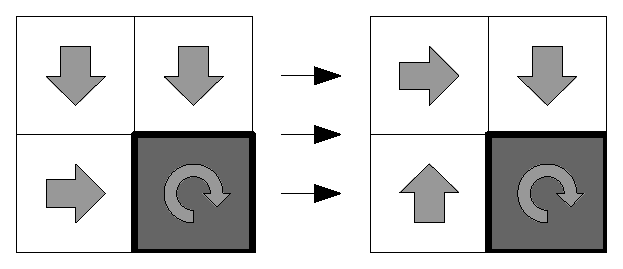
\psfig{file=img/envdopt.eps,width=5cm}}
\caption{\label{envdopt}The original optimal policy (left) and target policy (right).}
\end{figure}

Our experiments provided experimental verification of our proposed teaching method.  We verified that the method can be used both to speed up the learning process and tested this on policy iteration.  We also found that the method is able to direct the learner to a different policy by changing the dynamics of the environment.
